\documentclass[10pt,twocolumn,letterpaper]{article}

\usepackage{cvpr}
\usepackage{times}
\usepackage{epsfig}
\usepackage{graphicx}
\usepackage{amsmath}
\usepackage{amssymb}
\usepackage[normalem]{ulem}
\usepackage{textcomp}
\useunder{\uline}{\ul}{}
% Include other packages here, before hyperref.

% If you comment hyperref and then uncomment it, you should delete
% egpaper.aux before re-running latex.  (Or just hit 'q' on the first latex
% run, let it finish, and you should be clear).
\usepackage[breaklinks=true,bookmarks=false]{hyperref}

\cvprfinalcopy % *** Uncomment this line for the final submission

\def\cvprPaperID{****} % *** Enter the CVPR Paper ID here
\def\httilde{\mbox{\tt\raisebox{-.5ex}{\symbol{126}}}}

% Pages are numbered in submission mode, and unnumbered in camera-ready
%\ifcvprfinal\pagestyle{empty}\fi
\setcounter{page}{1}
\begin{document}

%%%%%%%%% TITLE
\title{Malaria Detection using Machine Learning}

\author{Harshit Goyal\\
{\tt\small harshit20203@iiitd.ac.in}
% For a paper whose authors are all at the same institution,
% omit the following lines up until the closing ``}''.
% Additional authors and addresses can be added with ``\and'',
% just like the second author.
% To save space, use either the email address or home page, not both
\and
Madhava Krishna\\
{\tt\small madhava20217@iiitd.ac.in}
\and
Shreya Bhatia\\
{\tt\small shreya20542@iiitd.ac.in}
\and
Srishti Singh\\
{\tt\small srishti20409@iiitd.ac.in}
}

\maketitle
%\thispagestyle{empty}

%%%%%%%%% ABSTRACT
\begin{abstract}
   Malaria is a life-threatening spread by infected Anopheles mosquito bites. Existing means of diagnosis include light microscopy and rapid diagnostic tests, which are used in conjuction to provide accurate results. However, the costs associated with them, in terms of human capital and time required, are immense.
   
   We seek to provide a complementing approach to infection classification using machine learning, which is fast and inexpensive. We examine the performance of algorithms like logistic regression, boosted decision trees, support vector machines and convolutional neural networks on cellular images, and the  effect of using image transformation and data augmentation approaches.

   Finally, we provide a GUI-based tool with a CNN model at its core to predict whether a given cell is parsitized or not.
\end{abstract}

%%%%%%%%% BODY TEXT
\section{Introduction}

Malaria is an infectious disease caused by 5 species of the Plasmodium parasite: \textit{Plasmodium falciparum}, \textit{Plasmodium vivax}, \textit{Plasmodium malariae}, \textit{Plasmodium ovale} and \textit{Plasmodium knowlesi}, spread by bites of the Anopheles mosquito. An estimated 241 million infections and 627,000 deaths occurred in 2020-21 \cite{worldmalaria}. 

\subsection{Testing Methods}
The infection can be detected using microscopy tests, Rapid Diagnostic Tests (RDTs) and serological tests.\cite{cdcmalaria}

Microscopy tests involve collecting and dyeing a thin or thick blood specimen with Giemsa or Wright's stain to detect infections visually and ascertain the percentage of infected to uninfected cells.

RDTs indicate whether the patient is infected with one of the species of the malaria-causing \textit{Plasmodium} and provide results in about 15 minutes. However, they fail to indicate a premature infection and negative RDT results need further evaluation. Using microscopy is also advised with positive results, so that the proportion of parasitized to uninfected cells can be determined.

Serological tests examine whether antibodies for the infection are present. They are mostly used for screening blood donors, testing for questionable diagnosis accompanied with treatment.

\subsection{Role of Machine Learning}
Numerous machine learning models have been proposed which segment a Whole Slide Image to identify red blood cells (RBCs) and classify these RBCs with a secondary trained model using deep neural network architectures and boosted trees. We observe how image transformations into the HSV mode can help isolate the irregularities better and propose models which can perform as well or better than existing ones.

\subsection{Colour Models}
Colour models are ways to represent colour images as tuples\cite{enwiki:1091166634}. A number of colour models have been proposed, each trying to capture a specific aspect of sight. The RGB colour model captures colours in Red, Green and Blue. The HSV colour space captures Hue, Saturation and Brightness. Saturation captures how pure the colour is\cite{Kurniastuti_2022}. Converting from RGB to HSV uses the following formula:

\begin{gather*}
   R' = R / 255\\
   G' = G / 255\\
   B' = B/255\\\\
C_{max} = \max(R', G', B')\\
C_{min} = \min(R', G', B')\\
\Delta = C_{max} - C{min} \\\\
\end{gather*}
\begin{align}
   H &= \begin{cases}
      0 & \Delta = 0\\
      60 \times (\frac{G' - B'}{\Delta}\mod{6}) & C_{max} = R'\\
      60 \times (\frac{B' - R'}{\Delta}+2) & C_{max} = G'\\
      60 \times (\frac{R' - G'}{\Delta} + 4)& C_{max} = B'
   \end{cases}\\
   S &= \begin{cases}
      0 & C_{max} = 0\\
      \frac{\Delta}{C_{max}} & C_{max} \neq 0
   \end{cases}\\
   V &= C_{max}
\end{align}

\section{Literature Survey}
%
Poostchi \etal created datasets, processed them, and tested a variety of algorithms like Naive Bayes, Logistic Regression, Decision Tree, Adaboost, SVMs, Neural Networks and Deep Neural Networks (DNNs). They also considered deployment of ML-based systems to diagnose Malaria \cite{POOSTCHI201836}.

Liang \etal. compared a 16-layer Convolutional Neural Network (CNN) model with transfer learning for classifying single infected cells. They noted that the CNN achieved greater accuracy, sensitivity, specificity, f1-score and Matthew's correlation coefficient over the latter \cite{7822567}.

Pan \etal explores preprocessing of images and segmentation to isolate single cells from wholeslide images. They used encoders and discussed encoder architectures for feature extraction, and discussed spatial and feature-space interpolation for enriching the dataset. They consistently noted higher performance of models trained on augmented datasets \cite{Pan18}.

Fuhad \etal implemented a CNN-based model and implemented data augmentation techniques like random rotations, zoom, translations, shear and horizontal flips. They used CNNs as an autoencoder to extract and reduce features and used SVM and KNN algorithms to classify the images. They conducted knowledge distillation in order to prune the trained model and reduce its complexity, and deployed the resulting commpressed model to mobile and web-based applications. They also conducted analyses if common mobile phones could utilize the model to classify cells. A final accuracy of 99.23\% was obtained by their efforts with a validation loss of 0.02 with the log loss function\cite{fuhadmalaria}.

\section{Dataset}
The dataset used was publicly available, courtesy of  images were taken at Chittagong Medical College Hospital, Bangladesh.\cite{datasetref}

\subsection{Dataset Description}
The dataset contains 13,799 parasitized and 13,799 uninfected image samples containing 3 colour dimensions for a total of 27,588 images. The images are of varying sizes. The maximum height and width was 385 and 394 pixels respectively. The minimum height are width was 40 and 46 pixels respectively. The mean height and width was 133 and 132 pixels respectively. The median height and width was 130 pixels. The mean aspect ratio of the images is 1.0138.

Out of the 27,588 images, 647 parasitized and 750 unparasitized images were misclassified \cite{fuhadmalaria}.

\begin{figure}[t]
   \begin{center}
      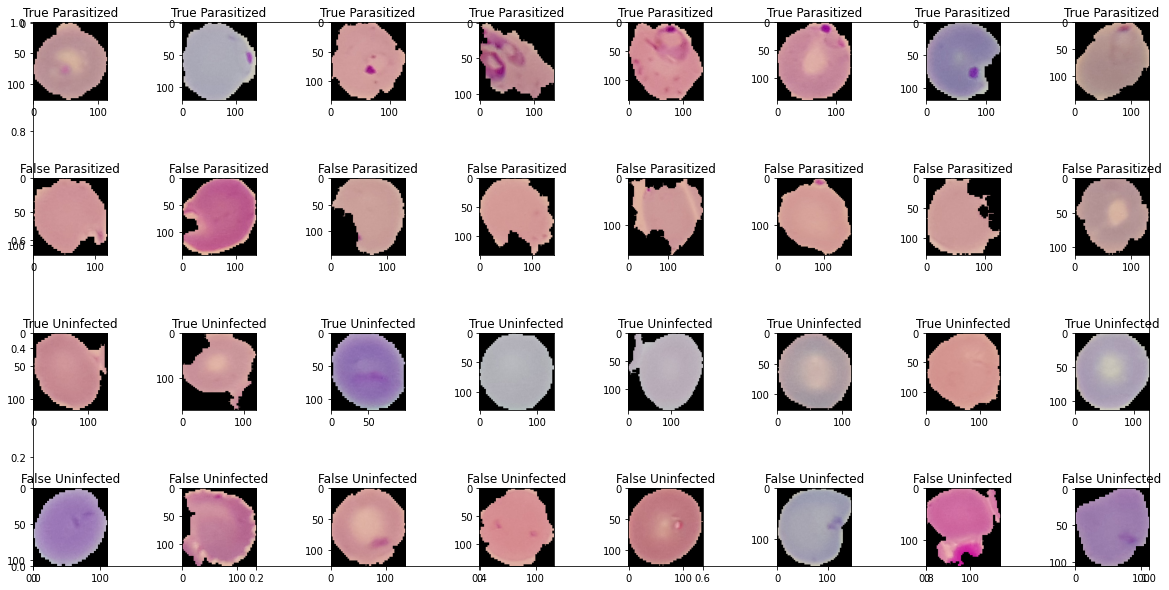
\includegraphics[width=1\linewidth]{../Plots/image_vis.png}
   \end{center}
      \caption{True and false parasitized and uninfected images.}
   \label{fig:malaria_image}
\end{figure}

\section{Methodology}

We adopted a modular approach and created modules designed for a specific task: data download and labelling, test-train-validation splits, model evaluation and data

\subsection{Exploratory Data Analysis}
In order to determine which colour channel was the clearest with respect to the identification of the chromatin dot characteristic to the parasitized cell, we plotted the images in different colour channels and in grayscale.

Out of the plotted images, the green channel showed the maximum isolation of the chromatin dot. We also visualised inverted images and noticed that the green channel had isolated the chromatin dot the most.
\begin{figure}[t]
   \begin{center}
      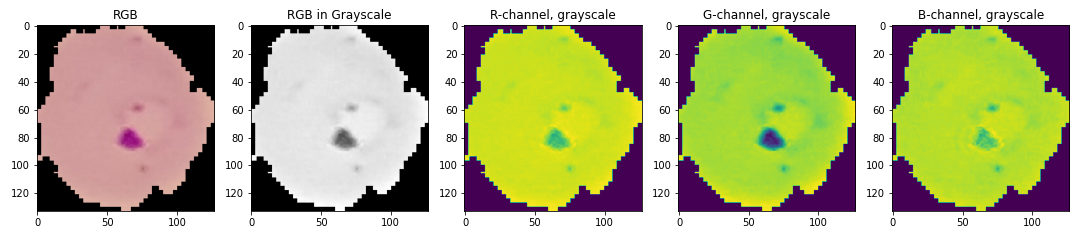
\includegraphics[width=1\linewidth]{../Plots/Comparison between channels.png}
   \end{center}
      \caption{Comparison between various colour channels for a true parasitized cell.}
   \label{fig:channel_comparison}
\end{figure}

We experimented with colour model transformations, and noticed that some models applying non-linear transformations (like HSV, HLS) captured the chromatin dot in parasitized cells better.

\begin{figure}[t]
   \begin{center}
      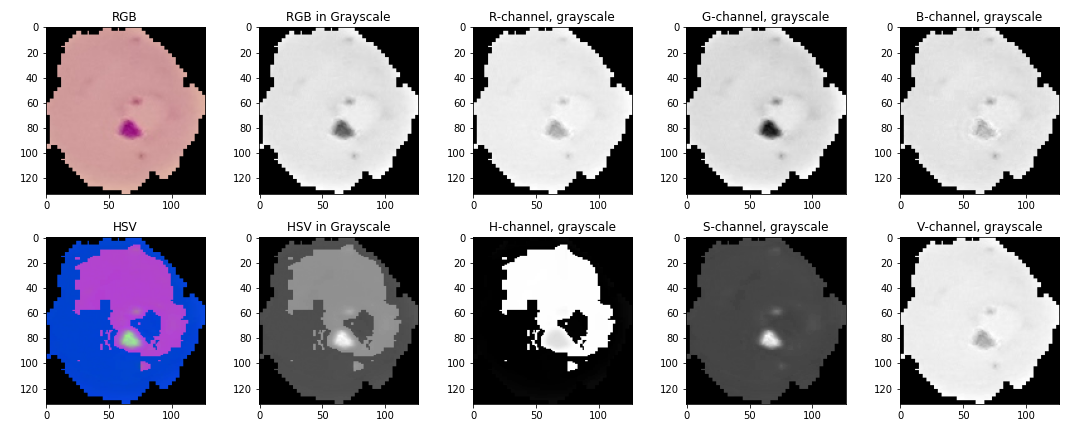
\includegraphics[width=1\linewidth]{../Plots/hsv_conversion.png}
   \end{center}
      \caption{Conversion to HSV space from RGB.}
   \label{fig:HSV_space}
\end{figure}

\subsubsection{Cluster Visualisation}
To visualise them, the images were first resized to a 50x50 colour format, each pixel value rescaled by 1/255, and each image finally flattened to a 50*50*3 length array. We used Euclidean distance as the distance metric and used the t-SNE algorithm to reduce dimensions to 2. We also used KMeans clustering to determine similarity clusters, but there was no clear relation between the natural clusters and the clusters output by K-Means (figure \ref{fig:tsne_vis}).

\begin{figure}[t]
   \begin{center}
      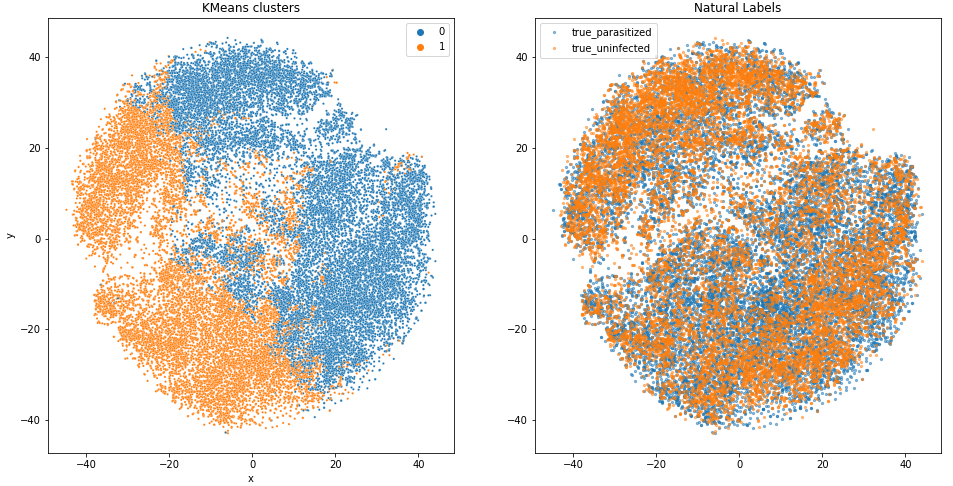
\includegraphics[width=1\linewidth]{../Plots/kmeans_natural labels.png}
   \end{center}
      \caption{KMeans and Natural Labels. The dataset was reduced to 2 dimensions using t-SNE.}
   \label{fig:tsne_vis}
\end{figure}

\subsection{Preprocessing}
The image data was read using Scikit-Image and each pixel value was scaled to a value between 0 and 1. The dimensions of each image were standardized to $25 \times 25$ to reduce computational complexity and VRAM requirements. Models were run using the standard RGB data which the datasets came in by default, and data transformed into the HSV format using Scikit-Image's $rgb2hsv$ function. Separate datasets were created and saved using Pickle for use. The datasets can be found \href{https://drive.google.com/drive/folders/1rKEHtQ_Sr2vU01yj_xC_ODwUp8QesxWY?usp=share_link}{here}.

\subsection{Data Augmentation}

We augmented images using the Albumentations package \cite{info11020125} and applied the following transformations on the training data:
\begin{enumerate}
   \item Rotation (range : -90\textdegree to +90\textdegree)
   \item Scaling: (range: 0.8 times to 1 times the original image size)
   \item Vertical Flip (probability = 0.5)
   \item Horizontal Flip (probability = 0.5)
   \item Shear (range: -7.5\textdegree to 7.5\textdegree)
   \item Gaussian Noise (Mean = 0, variance between 0.01 and 0.05)
\end{enumerate}

The augmentations were applied after rescaling to $25 \times 25$ image dimensions. The image was padded with zeroes after the transformations.

\subsection{Models}
The dataset was split in a stratified manner into training, validation and test sets. 80\% of the samples were used for the training, 10\% for validation and the last 10\% for testing. A random seed value was used while splitting for reproducible results.

Data augmentation was carried out by taking every image from the training set and generating two two randomly operated images, storing them in a separate array. 

The training dataset had 20,601 images, the augmented testing had 41,202 images, validation set had 2,943 images and the testing set had 2,617 images. The same augmented dataset was used for training all the augmented data models.

HSV conversion was carried out on all four datasets independently. As per the exploration and to reduce dimensionality, only the Saturation channel was used.

Hyperparameters were tuned on the validation set and the model parameters were unchanged between the unaugmented and augmented datasets. Early-stopping and checkpointing was used in TensorFlow-based models. The best-performing weights were loaded after the training completed.


\subsubsection{Naive Bayes}
We used Gaussian Naive Bayes without prior weight initialisation. Naive Bayes served as a baseline for classification, and as will be observed later, performed the worst consistently.

\subsubsection{Logistic regression}
Logistic Regression was implemented in TensorFlow using the Keras API. The Adam optimiser was used with learning rate tuned as per the performance on the validation set. 

\subsubsection{Decision trees}
Decision trees provide explainable modelling and are very fast to inference with. The maximum depth was adjusted depending on the performance on the validation set.

\subsubsection{XGBoost}
XGBoost with GPU-acceleration was used and a forest of 20 trees was created. The maximum depth was a hyperparmeter and tuned according to performance on the validation set.

\subsubsection{SVM}
SVM was implemented using Scikit-Learn's implementation. Polynomial kernel with a degree of 3 was used for classification (default parameters).

\subsubsection{CNNs}
A convolutional neural network was implemented in TensorFlow. The model architecture for the RGB and HSV datasets were different. The architecture of the CNN used for classifying the HSV images is shown in \ref{fig:cnn_architecture}

\begin{figure}[t]
   \begin{center}
      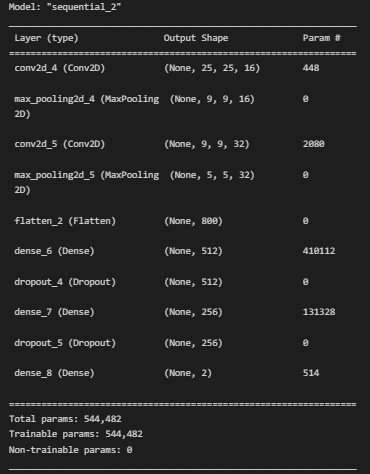
\includegraphics[width=1\linewidth]{../Plots/model_specifications.png}
   \end{center}
      \caption{CNN model architecture}
   \label{fig:cnn_architecture}
\end{figure}

\subsubsection{Transfer Learning}
We used the Xception model, trained on ImageNetperformed reasonably well. A resizing layer was added to the model which upscaled the dimension of the image to 72x72 from 25x25 to be compatible with the model. Unfortunately, the model required 3 input channels and it was not possible to use it for the HSV data.

\section{Results and Analysis}
The results are available in tables \ref{table:rgb_unaug}, \ref{table:rgb_aug}, \ref{table:hsv_unaug} and \ref{table:hsv_aug}.

We notice that among all models, the SVM model performs among the worst in all cases, followed by the Naive Bayes Classifier. It can be attributed to the classifier being unable to find a separating plane when the high dimensinal image data was compressed to the relatively low 3 dimensions.

Another striking thing we notice is that besides the logistic regression classifier, none of the models performed well on the RGB augmented data. This could have been a result of the nature of transformations used. Many attempts were made to regenerate the augmentations, but to no avail. We attempted to recreate the scenario using TensorFlow's ImageDataGenerator using the same data as inputs and the same transformations, but there was no difference in results in training the CNN model. The model failed to converge yet again and resulted in bad performance overall. We hypothesize that it is caused due to the selection of augmentation functions, but that remains to be tested.

The Saturation channel in the HSV conversion certainly made a noticeable impact. For the unaugmented dataset, the performance of the CNN and XGBoost increased, while that of Naive Bayes, Logistic Regression, Decision Tree, and SVM decreased. This is particularly interesting, as this gave us an almost 10\% performance increase for the XGBoost model and allowed the CNN model to match the accuracy of the top-performing models in this space.

Going from the unaugmented to augmented HSV dataset, we observe a general decline in performance, while that of the CNN increased (with the same model parameters). This surpasses previously proposed models with respect to the precision, recall and f1 scores, and is almost able to match them in terms of model accuracy.

The loss-curves for the CNN model can be seen in figures \ref{fig:cnn_rgb_losscurve}, \ref{fig:cnn_rgb_aug_losscurve}, \ref{fig:cnn_hsv_losscurve}, \ref{fig:cnn_hsv_aug_losscurve}. We notice some overfitting in \ref{fig:cnn_rgb_losscurve}, \ref{fig:cnn_hsv_losscurve}, and \ref{fig:cnn_hsv_aug_losscurve}, but the checkpointing and model reloading saves and reloads the best model, providing optimal results. Similar graphs were observed for the logistic learning and transfer-learning loss-curves.

Finally, we created a GUI-based interface which uses trained models for inferencing the class of a cell image. The video can be found \href{https://drive.google.com/file/d/1PuiOddcjlm_IbtReFyz8v2K37MM5XqCo/view?usp=share_link}{\textbf{here}}.

\begin{figure}[t]
   \begin{center}
      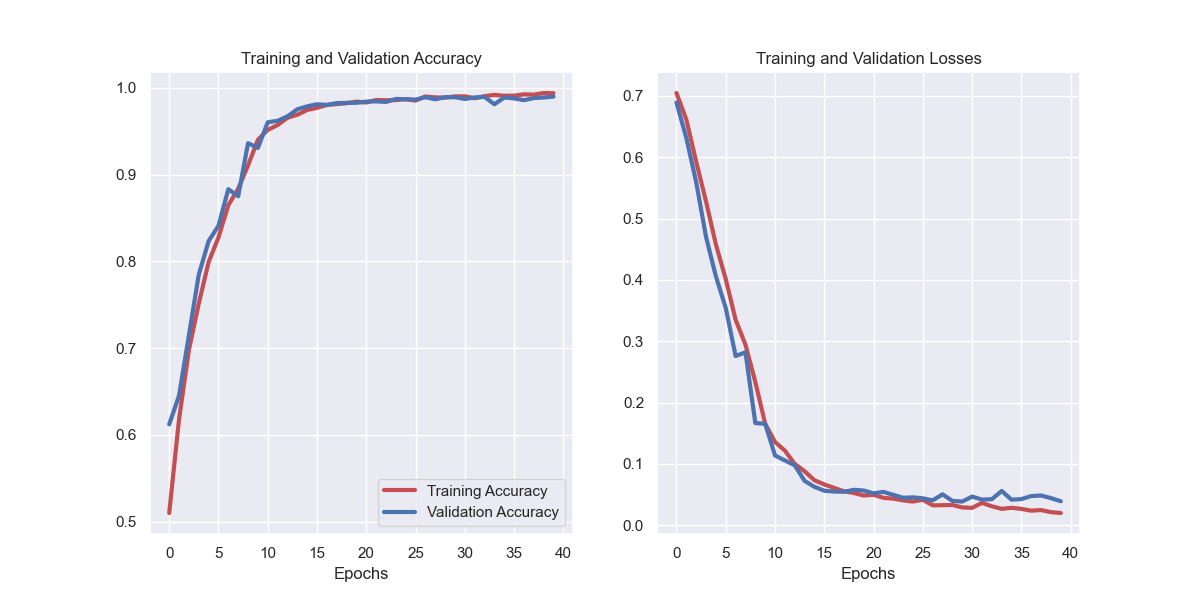
\includegraphics[width=1\linewidth]{../Plots/loss-curves/CNN_unaug_losscurve.png}
   \end{center}
      \caption{Loss-accuracy curve of the CNN model trained on unaugmented RGB data.}
   \label{fig:cnn_rgb_losscurve}
\end{figure}

\begin{figure}[t]
   \begin{center}
      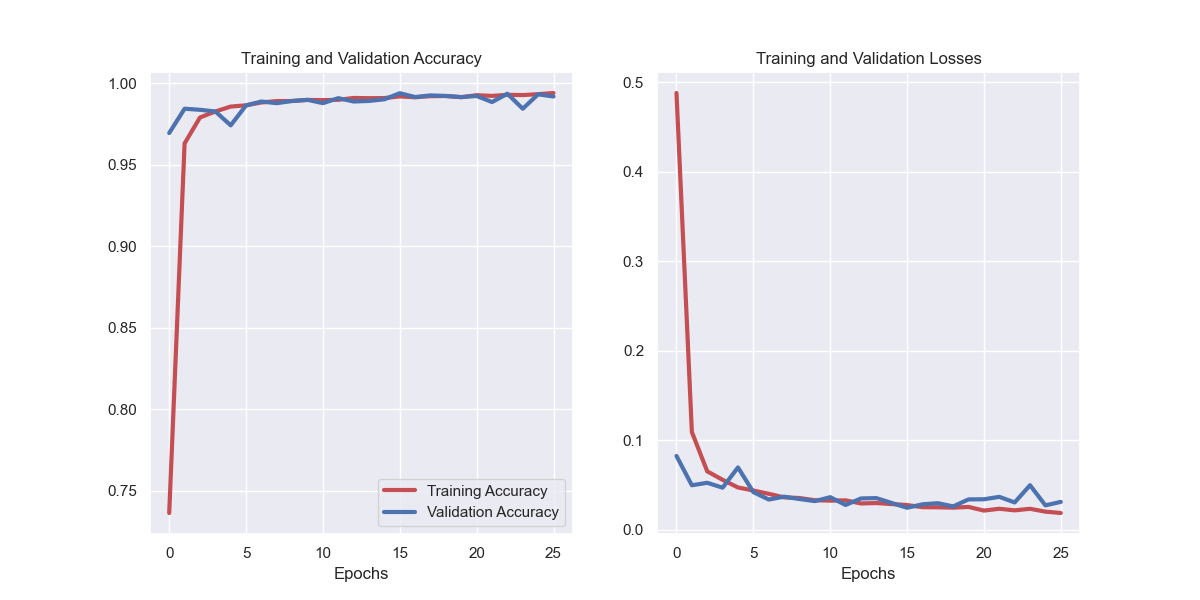
\includegraphics[width=1\linewidth]{../Plots/loss-curves/CNN_aug_losscurve.png}
   \end{center}
      \caption{Loss-accuracy curve of the CNN model trained on augmented RGB data.}
   \label{fig:cnn_rgb_aug_losscurve}
\end{figure}

\begin{figure}[t]
   \begin{center}
      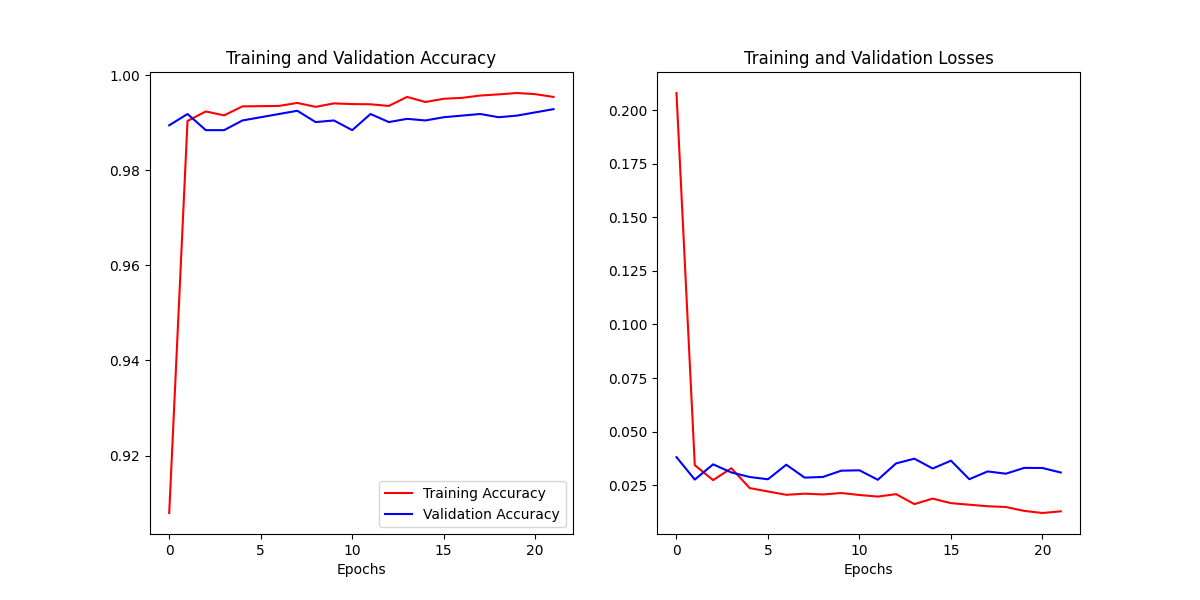
\includegraphics[width=1\linewidth]{../Plots/loss-curves/CNN_unaug_losscurve_HSV.png}
   \end{center}
      \caption{Loss-accuracy curve of the CNN model trained on unaugmented HSV data.}
   \label{fig:cnn_hsv_losscurve}
\end{figure}


\begin{figure}[t]
   \begin{center}
      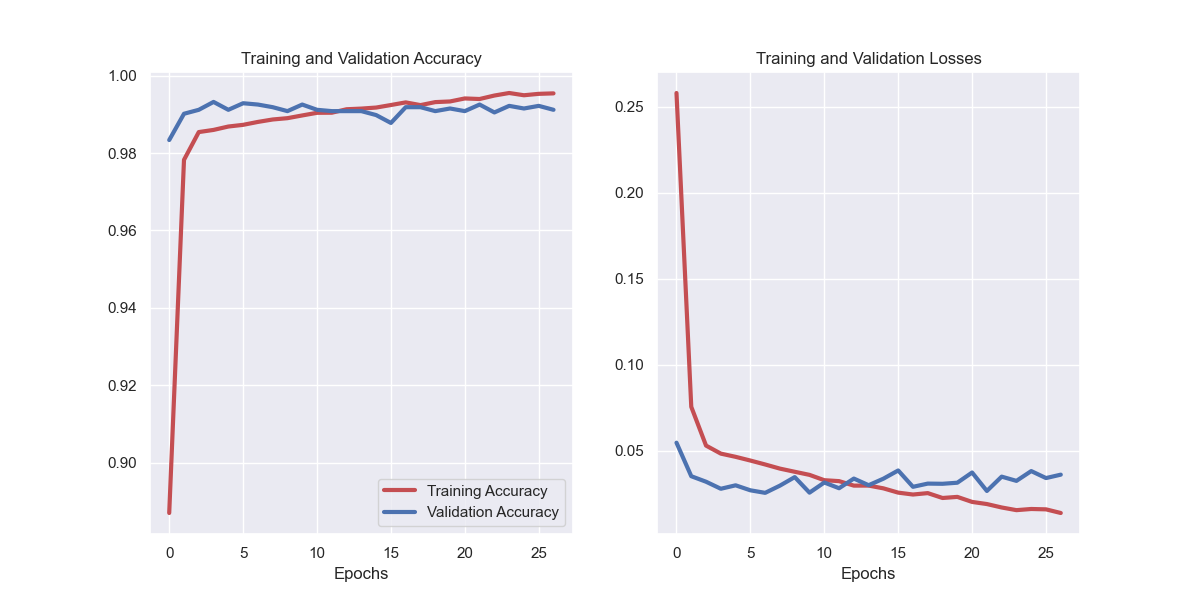
\includegraphics[width=1\linewidth]{../Plots/loss-curves/CNN_aug_losscurve_HSV.png}
   \end{center}
      \caption{Loss-accuracy curve of the CNN model trained on augmented HSV data.}
   \label{fig:cnn_hsv_aug_losscurve}
\end{figure}


\begin{table}[]
   \begin{tabular}{|lllll|}
   \hline
   \multicolumn{5}{|c|}{{\ul \textbf{RGB Unaugmented (Test Data)}}}                                                                                                  \\ \hline
   \multicolumn{1}{|l|}{{\ul Model}}   & \multicolumn{1}{l|}{{\ul Acc.}} & \multicolumn{1}{l|}{{\ul Prec.}} & \multicolumn{1}{l|}{{\ul Rec.}} & {\ul F1} \\ \hline
   \multicolumn{1}{|l|}{Naive Bayes}   & \multicolumn{1}{l|}{0.643}      & \multicolumn{1}{l|}{0.653}       & \multicolumn{1}{l|}{0.643}      & 0.638    \\ \hline
   \multicolumn{1}{|l|}{Logistic Regression}     & \multicolumn{1}{l|}{0.694}      & \multicolumn{1}{l|}{0.694}       & \multicolumn{1}{l|}{0.694}      & 0.694    \\ \hline
   \multicolumn{1}{|l|}{Decision Trees}            & \multicolumn{1}{l|}{0.684}      & \multicolumn{1}{l|}{0.687}       & \multicolumn{1}{l|}{0.684}      & 0.682    \\ \hline
   \multicolumn{1}{|l|}{XGBoost}       & \multicolumn{1}{l|}{0.850}      & \multicolumn{1}{l|}{0.850}       & \multicolumn{1}{l|}{0.850}      & 0.850    \\ \hline
   \multicolumn{1}{|l|}{SVM}           & \multicolumn{1}{l|}{0.518}      & \multicolumn{1}{l|}{0.550}       & \multicolumn{1}{l|}{0.516}      & 0.419    \\ \hline
   \multicolumn{1}{|l|}{Transfer Learning} & \multicolumn{1}{l|}{0.955}      & \multicolumn{1}{l|}{0.956}       & \multicolumn{1}{l|}{0.955}      & 0.955    \\ \hline
   \multicolumn{1}{|l|}{CNN}           & \multicolumn{1}{l|}{0.982}      & \multicolumn{1}{l|}{0.982}       & \multicolumn{1}{l|}{0.982}      & 0.982    \\ \hline
   \end{tabular}
   \caption{Performance of models trained on  RGB Unaugmented training data}
   \label{table:rgb_unaug}
\end{table}

\begin{table}[]
   \begin{tabular}{|lllll|}
   \hline
   \multicolumn{5}{|c|}{{\ul \textbf{RGB Augmented (Test Data)}}}                                                                                                            \\ \hline
   \multicolumn{1}{|l|}{{\ul Model}}         & \multicolumn{1}{l|}{{\ul Acc.}} & \multicolumn{1}{l|}{{\ul Prec.}} & \multicolumn{1}{l|}{{\ul Recall}} & {\ul F1} \\ \hline
   \multicolumn{1}{|l|}{Naive Bayes}         & \multicolumn{1}{l|}{0.502}      & \multicolumn{1}{l|}{0.251}       & \multicolumn{1}{l|}{0.500}        & 0.334    \\ \hline
   \multicolumn{1}{|l|}{Logistic Regression} & \multicolumn{1}{l|}{0.588}      & \multicolumn{1}{l|}{0.665}       & \multicolumn{1}{l|}{0.587}        & 0.532    \\ \hline
   \multicolumn{1}{|l|}{Decision Trees}      & \multicolumn{1}{l|}{0.502}      & \multicolumn{1}{l|}{0.251}       & \multicolumn{1}{l|}{0.500}        & 0.334    \\ \hline
   \multicolumn{1}{|l|}{XGBoost}             & \multicolumn{1}{l|}{0.498}      & \multicolumn{1}{l|}{0.249}       & \multicolumn{1}{l|}{0.500}        & 0.332    \\ \hline
   \multicolumn{1}{|l|}{SVM}                 & \multicolumn{1}{l|}{0.498}      & \multicolumn{1}{l|}{0.249}       & \multicolumn{1}{l|}{0.500}        & 0.332    \\ \hline
   \multicolumn{1}{|l|}{Transfer Learning}       & \multicolumn{1}{l|}{0.502}      & \multicolumn{1}{l|}{0.251}       & \multicolumn{1}{l|}{0.500}        & 0.334    \\ \hline
   \multicolumn{1}{|l|}{CNN}                 & \multicolumn{1}{l|}{0.502}      & \multicolumn{1}{l|}{0.251}       & \multicolumn{1}{l|}{0.500}        & 0.334    \\ \hline
   \end{tabular}
   \caption{Performance of models trained on augmented training data in the RGB domain.}
   \label{table:rgb_aug}
\end{table}

\begin{table}[]
   \begin{tabular}{|lllll|}
   \hline
   \multicolumn{5}{|c|}{{\ul \textbf{HSV Unaugmented (Test Data)}}}                                                                                                          \\ \hline
   \multicolumn{1}{|l|}{{\ul Model}}         & \multicolumn{1}{l|}{{\ul Acc.}} & \multicolumn{1}{l|}{{\ul Prec.}} & \multicolumn{1}{l|}{{\ul Recall}} & {\ul F1} \\ \hline
   \multicolumn{1}{|l|}{Naive Bayes}         & \multicolumn{1}{l|}{0.624}      & \multicolumn{1}{l|}{0.624}       & \multicolumn{1}{l|}{0.623}        & 0.623    \\ \hline
   \multicolumn{1}{|l|}{Logistic Regression} & \multicolumn{1}{l|}{0.677}      & \multicolumn{1}{l|}{0.677}       & \multicolumn{1}{l|}{0.677}        & 0.677    \\ \hline
   \multicolumn{1}{|l|}{Decision Trees}      & \multicolumn{1}{l|}{0.675}      & \multicolumn{1}{l|}{0.678}       & \multicolumn{1}{l|}{0.675}        & 0.674    \\ \hline
   \multicolumn{1}{|l|}{XGBoost}             & \multicolumn{1}{l|}{0.938}      & \multicolumn{1}{l|}{0.939}       & \multicolumn{1}{l|}{0.938}        & 0.938    \\ \hline
   \multicolumn{1}{|l|}{SVM}                 & \multicolumn{1}{l|}{0.502}      & \multicolumn{1}{l|}{0.251}       & \multicolumn{1}{l|}{0.500}        & 0.334    \\ \hline
   \multicolumn{1}{|l|}{CNN}                 & \multicolumn{1}{l|}{0.993}      & \multicolumn{1}{l|}{0.993}       & \multicolumn{1}{l|}{0.993}        & 0.993    \\ \hline
   \end{tabular}
   \caption{Performance of models trained on the saturation dimension training data converted into the HSV domain.}
   \label{table:hsv_unaug}
\end{table}


\begin{table}[]
   \begin{tabular}{|lllll|}
   \hline
   \multicolumn{5}{|c|}{{\ul \textbf{HSV Augmented (Test Data)}}}                                                                                                            \\ \hline
   \multicolumn{1}{|l|}{{\ul Model}}         & \multicolumn{1}{l|}{{\ul Acc.}} & \multicolumn{1}{l|}{{\ul Prec.}} & \multicolumn{1}{l|}{{\ul Recall}} & {\ul F1} \\ \hline
   \multicolumn{1}{|l|}{Naive Bayes}         & \multicolumn{1}{l|}{0.618}      & \multicolumn{1}{l|}{0.624}       & \multicolumn{1}{l|}{0.617}        & 0.611    \\ \hline
   \multicolumn{1}{|l|}{Logistic Regression} & \multicolumn{1}{l|}{0.625}      & \multicolumn{1}{l|}{0.627}       & \multicolumn{1}{l|}{0.625}        & 0.623    \\ \hline
   \multicolumn{1}{|l|}{Decision Trees}      & \multicolumn{1}{l|}{0.789}      & \multicolumn{1}{l|}{0.819}       & \multicolumn{1}{l|}{0.789}        & 0.784    \\ \hline
   \multicolumn{1}{|l|}{XGBoost}             & \multicolumn{1}{l|}{0.930}      & \multicolumn{1}{l|}{0.931}       & \multicolumn{1}{l|}{0.930}        & 0.930    \\ \hline
   \multicolumn{1}{|l|}{SVM}                 & \multicolumn{1}{l|}{0.501}      & \multicolumn{1}{l|}{0.251}       & \multicolumn{1}{l|}{0.499}        & 0.334    \\ \hline
   \multicolumn{1}{|l|}{CNN}                 & \multicolumn{1}{l|}{0.994}      & \multicolumn{1}{l|}{0.994}       & \multicolumn{1}{l|}{0.994}        & 0.994    \\ \hline
   \end{tabular}
   \caption{Performance of models trained on the saturation domain of augmented images converted to the HSV domain.}
   \label{table:hsv_aug}
   \end{table}

\section{Conclusion}
%TODO
We first notice the sheer strength of the CNN-based models. They are consistently at the top of the charts (excepting the outlier RGB-augmented data, on which no model could get properly trained).

We also notice that the HSV colour transformation helps with the CNN and XGBoost models, both of which shot up in accuracy significantly. The XGBoost model is said to be a powerful tool and it made it clear here.

The role of augmentations remains vague with the amount of testing done so far, with CNN models performing slightly better than before using them, but not by a significant margin. The values and kinds of transformations used for augmenting the data must be carefully determined so as to prohibit scenarios like the lack of convergence.


%-------------------------------------------------------------------------
% \subsection{Language}

% All manuscripts must be in English.

% \subsection{Dual submission}

% Please refer to the author guidelines on the CVPR 2020 web page for a
% discussion of the policy on dual submissions.

% \subsection{Paper length}
% Papers, excluding the references section,
% must be no longer than eight pages in length. The references section
% will not be included in the page count, and there is no limit on the
% length of the references section. For example, a paper of eight pages
% with two pages of references would have a total length of 10 pages.
% {\bf There will be no extra page charges for CVPR 2020.}

% Overlength papers will simply not be reviewed.  This includes papers
% where the margins and formatting are deemed to have been significantly
% altered from those laid down by this style guide.  Note that this
% \LaTeX\ guide already sets figure captions and references in a smaller font.
% The reason such papers will not be reviewed is that there is no provision for
% supervised revisions of manuscripts.  The reviewing process cannot determine
% the suitability of the paper for presentation in eight pages if it is
% reviewed in eleven.  

% %-------------------------------------------------------------------------
% \subsection{The ruler}
% The \LaTeX\ style defines a printed ruler which should be present in the
% version submitted for review.  The ruler is provided in order that
% reviewers may comment on particular lines in the paper without
% circumlocution.  If you are preparing a document using a non-\LaTeX\
% document preparation system, please arrange for an equivalent ruler to
% appear on the final output pages.  The presence or absence of the ruler
% should not change the appearance of any other content on the page.  The
% camera ready copy should not contain a ruler. (\LaTeX\ users may uncomment
% the \verb'\cvprfinalcopy' command in the document preamble.)  Reviewers:
% note that the ruler measurements do not align well with lines in the paper
% --- this turns out to be very difficult to do well when the paper contains
% many figures and equations, and, when done, looks ugly.  Just use fractional
% references (e.g.\ this line is $095.5$), although in most cases one would
% expect that the approximate location will be adequate.

% \subsection{Mathematics}

% Please number all of your sections and displayed equations.  It is
% important for readers to be able to refer to any particular equation.  Just
% because you didn't refer to it in the text doesn't mean some future reader
% might not need to refer to it.  It is cumbersome to have to use
% circumlocutions like ``the equation second from the top of page 3 column
% 1''.  (Note that the ruler will not be present in the final copy, so is not
% an alternative to equation numbers).  All authors will benefit from reading
% Mermin's description of how to write mathematics:
% \url{http://www.pamitc.org/documents/mermin.pdf}.


% \subsection{Blind review}

% Many authors misunderstand the concept of anonymizing for blind
% review.  Blind review does not mean that one must remove
% citations to one's own work---in fact it is often impossible to
% review a paper unless the previous citations are known and
% available.

% Blind review means that you do not use the words ``my'' or ``our''
% when citing previous work.  That is all.  (But see below for
% techreports.)

% Saying ``this builds on the work of Lucy Smith [1]'' does not say
% that you are Lucy Smith; it says that you are building on her
% work.  If you are Smith and Jones, do not say ``as we show in
% [7]'', say ``as Smith and Jones show in [7]'' and at the end of the
% paper, include reference 7 as you would any other cited work.

% An example of a bad paper just asking to be rejected:
% \begin{quote}
% \begin{center}
%     An analysis of the frobnicatable foo filter.
% \end{center}

%    In this paper we present a performance analysis of our
%    previous paper [1], and show it to be inferior to all
%    previously known methods.  Why the previous paper was
%    accepted without this analysis is beyond me.

%    [1] Removed for blind review
% \end{quote}


% An example of an acceptable paper:

% \begin{quote}
% \begin{center}
%      An analysis of the frobnicatable foo filter.
% \end{center}

%    In this paper we present a performance analysis of the
%    paper of Smith \etal [1], and show it to be inferior to
%    all previously known methods.  Why the previous paper
%    was accepted without this analysis is beyond me.

%    [1] Smith, L and Jones, C. ``The frobnicatable foo
%    filter, a fundamental contribution to human knowledge''.
%    Nature 381(12), 1-213.
% \end{quote}

% If you are making a submission to another conference at the same time,
% which covers similar or overlapping material, you may need to refer to that
% submission in order to explain the differences, just as you would if you
% had previously published related work.  In such cases, include the
% anonymized parallel submission~\cite{cdcmalaria} as additional material and
% cite it as
% \begin{quote}
% [1] Authors. ``The frobnicatable foo filter'', F\&G 2014 Submission ID 324,
% Supplied as additional material {\tt fg324.pdf}.
% \end{quote}

% Finally, you may feel you need to tell the reader that more details can be
% found elsewhere, and refer them to a technical report.  For conference
% submissions, the paper must stand on its own, and not {\em require} the
% reviewer to go to a techreport for further details.  Thus, you may say in
% the body of the paper ``further details may be found
% in~\cite{Authors14b}''.  Then submit the techreport as additional material.
% Again, you may not assume the reviewers will read this material.

% Sometimes your paper is about a problem which you tested using a tool which
% is widely known to be restricted to a single institution.  For example,
% let's say it's 1969, you have solved a key problem on the Apollo lander,
% and you believe that the CVPR70 audience would like to hear about your
% solution.  The work is a development of your celebrated 1968 paper entitled
% ``Zero-g frobnication: How being the only people in the world with access to
% the Apollo lander source code makes us a wow at parties'', by Zeus \etal.

% You can handle this paper like any other.  Don't write ``We show how to
% improve our previous work [Anonymous, 1968].  This time we tested the
% algorithm on a lunar lander [name of lander removed for blind review]''.
% That would be silly, and would immediately identify the authors. Instead
% write the following:
% \begin{quotation}
% \noindent
%    We describe a system for zero-g frobnication.  This
%    system is new because it handles the following cases:
%    A, B.  Previous systems [Zeus et al. 1968] didn't
%    handle case B properly.  Ours handles it by including
%    a foo term in the bar integral.

%    ...

%    The proposed system was integrated with the Apollo
%    lunar lander, and went all the way to the moon, don't
%    you know.  It displayed the following behaviours
%    which show how well we solved cases A and B: ...
% \end{quotation}
% As you can see, the above text follows standard scientific convention,
% reads better than the first version, and does not explicitly name you as
% the authors.  A reviewer might think it likely that the new paper was
% written by Zeus \etal, but cannot make any decision based on that guess.
% He or she would have to be sure that no other authors could have been
% contracted to solve problem B.
% \medskip

% \noindent
% FAQ\medskip\\
% {\bf Q:} Are acknowledgements OK?\\
% {\bf A:} No.  Leave them for the final copy.\medskip\\
% {\bf Q:} How do I cite my results reported in open challenges?
% {\bf A:} To conform with the double blind review policy, you can report results of other challenge participants together with your results in your paper. For your results, however, you should not identify yourself and should not mention your participation in the challenge. Instead present your results referring to the method proposed in your paper and draw conclusions based on the experimental comparison to other results.\medskip\\



% % \begin{figure}[t]
% % \begin{center}
% % \fbox{\rule{0pt}{2in} \rule{0.9\linewidth}{0pt}}
% %    %\includegraphics[width=0.8\linewidth]{egfigure.eps}
% % \end{center}
% %    \caption{Example of caption.  It is set in Roman so that mathematics
% %    (always set in Roman: $B \sin A = A \sin B$) may be included without an
% %    ugly clash.}
% % \label{fig:long}
% % \label{fig:onecol}
% % \end{figure}

% \subsection{Miscellaneous}

% \noindent
% Compare the following:\\
% \begin{tabular}{ll}
%  \verb'$conf_a$' &  $conf_a$ \\
%  \verb'$\mathit{conf}_a$' & $\mathit{conf}_a$
% \end{tabular}\\
% See The \TeX book, p165.

% The space after \eg, meaning ``for example'', should not be a
% sentence-ending space. So \eg is correct, {\em e.g.} is not.  The provided
% \verb'\eg' macro takes care of this.

% When citing a multi-author paper, you may save space by using ``et alia'',
% shortened to ``\etal'' (not ``{\em et.\ al.}'' as ``{\em et}'' is a complete word.)
% However, use it only when there are three or more authors.  Thus, the
% following is correct: ``
%    Frobnication has been trendy lately.
%    It was introduced by Alpher~\cite{Alpher02}, and subsequently developed by
%    Alpher and Fotheringham-Smythe~\cite{Alpher03}, and Alpher \etal~\cite{Alpher04}.''

% This is incorrect: ``... subsequently developed by Alpher \etal~\cite{Alpher03} ...''
% because reference~\cite{Alpher03} has just two authors.  If you use the
% \verb'\etal' macro provided, then you need not worry about double periods
% when used at the end of a sentence as in Alpher \etal.

% For this citation style, keep multiple citations in numerical (not
% chronological) order, so prefer \cite{Alpher03,Alpher02,cdcmalaria} to
% \cite{Alpher02,Alpher03,cdcmalaria}.


% % \begin{figure*}
% % \begin{center}
% % \fbox{\rule{0pt}{2in} \rule{.9\linewidth}{0pt}}
% % \end{center}
% %    \caption{Example of a short caption, which should be centered.}
% % \label{fig:short}
% % \end{figure*}

% %------------------------------------------------------------------------
% \section{Formatting your paper}

% All text must be in a two-column format. The total allowable width of the
% text area is $6\frac78$ inches (17.5 cm) wide by $8\frac78$ inches (22.54
% cm) high. Columns are to be $3\frac14$ inches (8.25 cm) wide, with a
% $\frac{5}{16}$ inch (0.8 cm) space between them. The main title (on the
% first page) should begin 1.0 inch (2.54 cm) from the top edge of the
% page. The second and following pages should begin 1.0 inch (2.54 cm) from
% the top edge. On all pages, the bottom margin should be 1-1/8 inches (2.86
% cm) from the bottom edge of the page for $8.5 \times 11$-inch paper; for A4
% paper, approximately 1-5/8 inches (4.13 cm) from the bottom edge of the
% page.

% %-------------------------------------------------------------------------
% \subsection{Margins and page numbering}

% All printed material, including text, illustrations, and charts, must be kept
% within a print area 6-7/8 inches (17.5 cm) wide by 8-7/8 inches (22.54 cm)
% high.
% Page numbers should be in footer with page numbers, centered and .75
% inches from the bottom of the page and make it start at the correct page
% number rather than the 4321 in the example.  To do this fine the line (around
% line 23)
% \begin{verbatim}
% %\ifcvprfinal\pagestyle{empty}\fi
% \setcounter{page}{4321}
% \end{verbatim}
% where the number 4321 is your assigned starting page.

% Make sure the first page is numbered by commenting out the first page being
% empty on line 46
% \begin{verbatim}
% %\thispagestyle{empty}
% \end{verbatim}


% %-------------------------------------------------------------------------
% \subsection{Type-style and fonts}

% Wherever Times is specified, Times Roman may also be used. If neither is
% available on your word processor, please use the font closest in
% appearance to Times to which you have access.

% MAIN TITLE. Center the title 1-3/8 inches (3.49 cm) from the top edge of
% the first page. The title should be in Times 14-point, boldface type.
% Capitalize the first letter of nouns, pronouns, verbs, adjectives, and
% adverbs; do not capitalize articles, coordinate conjunctions, or
% prepositions (unless the title begins with such a word). Leave two blank
% lines after the title.

% AUTHOR NAME(s) and AFFILIATION(s) are to be centered beneath the title
% and printed in Times 12-point, non-boldface type. This information is to
% be followed by two blank lines.

% The ABSTRACT and MAIN TEXT are to be in a two-column format.

% MAIN TEXT. Type main text in 10-point Times, single-spaced. Do NOT use
% double-spacing. All paragraphs should be indented 1 pica (approx. 1/6
% inch or 0.422 cm). Make sure your text is fully justified---that is,
% flush left and flush right. Please do not place any additional blank
% lines between paragraphs.

% Figure and table captions should be 9-point Roman type as in
% Figures~\ref{fig:onecol} and~\ref{fig:short}.  Short captions should be centred.

% \noindent Callouts should be 9-point Helvetica, non-boldface type.
% Initially capitalize only the first word of section titles and first-,
% second-, and third-order headings.

% FIRST-ORDER HEADINGS. (For example, {\large \bf 1. Introduction})
% should be Times 12-point boldface, initially capitalized, flush left,
% with one blank line before, and one blank line after.

% SECOND-ORDER HEADINGS. (For example, { \bf 1.1. Database elements})
% should be Times 11-point boldface, initially capitalized, flush left,
% with one blank line before, and one after. If you require a third-order
% heading (we discourage it), use 10-point Times, boldface, initially
% capitalized, flush left, preceded by one blank line, followed by a period
% and your text on the same line.

% %-------------------------------------------------------------------------
% \subsection{Footnotes}

% Please use footnotes\footnote {This is what a footnote looks like.  It
% often distracts the reader from the main flow of the argument.} sparingly.
% Indeed, try to avoid footnotes altogether and include necessary peripheral
% observations in
% the text (within parentheses, if you prefer, as in this sentence).  If you
% wish to use a footnote, place it at the bottom of the column on the page on
% which it is referenced. Use Times 8-point type, single-spaced.


% %-------------------------------------------------------------------------
% \subsection{References}

% List and number all bibliographical references in 9-point Times,
% single-spaced, at the end of your paper. When referenced in the text,
% enclose the citation number in square brackets, for
% example~\cite{cdcmalaria}.  Where appropriate, include the name(s) of
% editors of referenced books.

% \begin{table}
% \begin{center}
% \begin{tabular}{|l|c|}
% \hline
% Method & Frobnability \\
% \hline\hline
% Theirs & Frumpy \\
% Yours & Frobbly \\
% Ours & Makes one's heart Frob\\
% \hline
% \end{tabular}
% \end{center}
% \caption{Results.   Ours is better.}
% \end{table}

% %-------------------------------------------------------------------------
% \subsection{Illustrations, graphs, and photographs}

% All graphics should be centered.  Please ensure that any point you wish to
% make is resolvable in a printed copy of the paper.  Resize fonts in figures
% to match the font in the body text, and choose line widths which render
% effectively in print.  Many readers (and reviewers), even of an electronic
% copy, will choose to print your paper in order to read it.  You cannot
% insist that they do otherwise, and therefore must not assume that they can
% zoom in to see tiny details on a graphic.

% When placing figures in \LaTeX, it's almost always best to use
% \verb+\includegraphics+, and to specify the  figure width as a multiple of
% the line width as in the example below
% {\small\begin{verbatim}
%    \usepackage[dvips]{graphicx} ...
%    \includegraphics[width=0.8\linewidth]
%                    {myfile.eps}
% \end{verbatim}
% }


% %-------------------------------------------------------------------------
% \subsection{Color}

% Please refer to the author guidelines on the CVPR 2020 web page for a discussion
% of the use of color in your document.

% %------------------------------------------------------------------------
% \section{Final copy}

% You must include your signed IEEE copyright release form when you submit
% your finished paper. We MUST have this form before your paper can be
% published in the proceedings.

% Please direct any questions to the production editor in charge of these 
% proceedings at the IEEE Computer Society Press: 
% \url{https://www.computer.org/about/contact}. 


{\small
\bibliographystyle{ieeetr}
\bibliography{egbib}
}

\end{document}
